\section{Filled vertex groups and central panels}\label{sec:09-fans}

Fix a terminal folded vertex row $J=Y_v$.  We construct the first
pieces of the walls used to cubulate its induced filling $\bar J$.
The relative subgroups of $J$ are denoted by $P$: they comprise the
included height kernels $P_d=S_d$, the external cyclic intersections,
and the intersections with the additional maximal cyclic family in the
root case.  All subgroup notation includes the specified conjugations
and coset occurrences.  The relative-row results of
Section~\ref{sec:07-transfer} and the kernels of
Section~\ref{sec:08-kernels} are used throughout.  In particular, the
standalone filling has exact peripheral reductions, its relative
hyperbolicity constants are uniform, and all finitely many prescribed
injection, membership, and coset-avoidance tests can be imposed before
filling.  There are finitely many row and incidence types.  Every choice
in this section is made simultaneously for those types.

Here is the local construction we seek. Free-group Cayley trees supply
horizontal edges, whose original vertices are called ordinary sites.
A vertex representing a peripheral coset is called an apex. After filling,
its central incidences form a finite
link graph: link vertices index radial edges to ordinary sites, and link
edges record horizontal edges between those sites. Binary labels on the
link vertices prescribe radial cochain values. Where the labels change,
the intervening horizontal edge must have mod-two cochain total one. We
match these cut marks at copies of shared horizontal midpoints. Large
angles between the corresponding radial edges will make the matched
components quasiconvex trees.
We first identify the central incidences and their cyclic attachments,
then build the fan model in which this matching takes place. The exact
covers from the preceding section supply the binary labels; the next
section extends their cochains across the cyclic attachments by cancelling
odd boundary totals.

\subsection{The central components before filling}

\begin{lemma}[The component presentation]\label{fan:components}
The developed presentation of $J$ can be arranged as a tree of central
components with the following properties.
\begin{enumerate}[label=\textup{(\roman*)}]
\item A central component has a bipartite tree of groups, with finite-rank
free groups $F$ at one class of nodes and internal peripheral groups
$P_d$ at the other.  Each incidence group is a nontrivial finitely
generated subgroup $M\le P_d$ embedded in its neighboring $F$.
\item Each edge between central components has infinite cyclic group
$\langle c\rangle$.  At one end it attaches to an internal node $d$;
at the other it attaches in a different central component.  Distinct
outgoing incidences at the same $d$ have distinct target components.
\item The unused relative occurrences are cyclic.  We call them outer
occurrences.  Internal and outer nodes together label the actual
peripheral cosets, without duplication.  The developed data have finite
quotient by $J$.
\end{enumerate}
Every included $S_d$ has a central incidence.  The added cyclic root
nodes have their root incidences.  Elementary filled rows may be omitted
from the wall construction.
\end{lemma}

\begin{proof}
There are three cases.

For a free actual row $X_x$, use the incidence tree $\Gamma_v$ itself.
Its actual nodes carry free groups, its object nodes carry the included
$S_d$, and its edges carry $M_x^d$.  These are the central data; the
remaining relative groups are outer cyclics.

Suppose next that the actual row has a nonfree root, and choose one of
its slots.  Write the root splitting, with all translates understood, as
\[
 E*_{\langle z\rangle=\langle u^a\rangle} U,
 \qquad U=\langle u\rangle,
\]
where $E$ is free. Its Bass--Serre tree is the root tree used below.
First assume that powers of the root group are hit by the strict object
system. The root case in the proof of
Proposition~\ref{close:folded-slot} gives
$\widetilde F=X_x\cap Y_f=X_x$: all actual edges of the chosen slot above $x$ go to
one folded edge $f$.  Each object node $d$ likewise belongs to a unique
$K_f$.  Consequently the subtrees $K_f\subset\Gamma_v$ partition its
vertices into connected subtrees.  An incidence $(x,d)$ belongs to its
partition subtree precisely when $M_x^d$ meets an $E$-node of the root
tree nontrivially.  This uses the identification of $K_f$ with the actual
incidence image of $\Gamma_f$, together with
Lemma~\ref{close:strict-subtrees}, which puts every nontrivial actual
incidence in the enlarged $Z_d$.

A missing incidence therefore has cyclic group $M_x^d$ acting
hyperbolically on the root tree. Indeed, the local homology equality in
Lemma~\ref{close:strict-subtrees}, inherited from
Proposition~\ref{row:period-rule}, forces
a noncyclic incidence group to meet an $E$-node, whereas an elliptic
cyclic incidence meets such a node after passing to a nonzero power.
Collapse the $K_f$.  The component stabilizer is $Y_f$, whose developed
presentation $\Gamma_f$ has free groups $E_e$, full object groups
$P_d=S_d$, and incidence groups $M_e^d$.  A missing edge joins different
components: it injects into $P_d$ at one end and into
$X_x\le Y_f$ at the other.  Collapsing disjoint subtrees of a tree gives
a tree, so two missing edges at a fixed $d$ cannot lead to the same
component.

Finally suppose that root powers are unclaimed.  The additional
maximal cyclic family $U^*$ is then disjoint from the old object system.
For the action of $M_x^d$ on the root tree, edge-group and cyclic-node
intersections are trivial. The no-hit case of
Proposition~\ref{close:folded-slot} identifies the direct sum of the
first homologies of its free-node intersections with $H_1(M_x^d)$,
over the ambient division field. The tree Mayer sequence now has the
following consequence: either $M_x^d$ is cyclic and acts hyperbolically,
or it is contained in one free-node stabilizer.  If all free-node
intersections are trivial, the action is free and $M_x^d$ is a
finitely generated free group.  Its first division-field homology
has dimension $\rk(M_x^d)-1$; the period rule makes this zero, so its
nontriviality forces rank one.  To see the other alternative explicitly, the quotient graph of groups has trivial edge
groups.  If it had two nontrivial vertex-group orbits, or a nontrivial
free graph factor in addition to one such orbit, the degree-zero edge
term would contribute additional first homology.  Thus, when a
free-node intersection is nontrivial, there is one such orbit, no
additional free factor, and the whole group fixes that free node.  The
fixed free node is unique because intervening root edges have trivial
$M_x^d$-stabilizer.

Cut $\Gamma_v$ along the cyclic hyperbolic incidences and expand the
remaining actual nodes by their root trees.  Attach every other
incidence to its unique free node.  Both the $S_d$-nodes and the cyclic
$U$-nodes are internal.  A $U$-node represents a distinct $U^*$-occurrence
whose intersection with $J$ is exactly $U$: a nonzero root power fixes
only this actual $x$ in $\Gamma_v$, since it fixes no object node, and
the root cyclic stabilizers inside $X_x$ are distinct maximal cyclics.
An element in the same maximal cyclic group must preserve this unique
$x$, so it belongs to the indicated root cyclic stabilizer.  The same
argument shows that different developed $U$-nodes cannot represent the
same peripheral occurrence.  The root incidences have group
$\langle u^a\rangle$; the incidences at $S_d$ are the actual row
intersections.  The cut edges again join an $S_d$-node to a different
component, with their other map landing in $X_x$.

In all three cases the preceding cocompactness results give finite
quotient data.  Positive period dimension at a free level supplies a
central incidence at every included $S_d$.  The incidences at cyclic
root nodes are displayed in the root splitting.  This proves the
assertions.
\end{proof}

\subsection{A tagged fan complex}

Build a $J$-complex $\mathcal X$ from the presentation in
Lemma~\ref{fan:components}.  Its edge graph is given unit edge lengths.
The following tags are part of the construction, even when two cells
have the same image or the same endpoints.

\begin{enumerate}[label=\textup{(\arabic*)}]
\item At a free node use its Cayley tree for a finite free basis.
Subdivide each positive oriented edge by a midpoint.  The original
vertices are \emph{ordinary sites}; the two subdivided edges are
\emph{horizontal half-edges}.  For an incidence group $M$, use its
minimal invariant subtree, namely the lift of an unbased finite
Stallings core immersion \cite[Sections~3, 5 and~7]{Stallings1983}.
Cone this subtree from its internal apex
$d$, with spokes to ordinary vertices and midpoints and with a triangle
over every horizontal half-edge.  The resulting central complex may
have several connected components.
\item For a component edge with group $\langle c\rangle\le P_d$, choose
a central word path in its target component from an ordinary site to
its $c$-translate.  Repeat it on an abstract indexed line and cone that
line from $d$.  This is a \emph{satellite arm}.  Choices are made on
representatives of developed component-edge orbits and then extended
equivariantly.  The cyclic group acts on the indexed line by
translation; consequently no further compatibility inside the target
$X_x$ is required.  The boundary path is allowed to repeat vertices or
edges, but each spoke and each fan triangle retains its occurrence tag.
We choose the path so that every apex neighbor on it is ordinary and
every midpoint neighbor is a true ordinary endpoint of its horizontal
edge.  Horizontal edges and these radial edges already connect the
central components.  The complex after this step is called internal.
\item For an outer occurrence $p$, with $P_p=\langle c_p\rangle$, choose
in the internal complex a word path from an ordinary site to its
$c_p$-translate.  Cone the repeated indexed path from a new apex $p$,
again retaining all tags.  Use the same ordinary-neighbor convention
at internal apices and midpoints.
\end{enumerate}

Each central component is simply connected: it is a tree of simply
connected free-node spaces, point spaces, and incidence subtrees.  The
satellite construction joins these components along their component
tree.  Each joining slab is the mapping cylinder of its indexed line's
boundary map, with the other end collapsed to its source point.
Van Kampen's theorem therefore preserves simple connectivity.  Coning
the remaining outer indexed lines preserves it as well.

There are finitely many cell types modulo $J$.  Apex vertices are
exactly the marked peripheral cosets; all other vertices and all
oriented edges have free $J$-action.  In particular an oriented edge of
a fixed type has a regular frame $g\in J$, and its endpoints have forms
\begin{equation}\label{fan:frame-formula}
 gt\quad\hbox{or}\quad gtP
\end{equation}
for fixed offsets $t$ depending only on the endpoint and edge type.
For satellite and outer spokes, freeness follows from the indexed-line
tags, rather than from injectivity of the boundary path. The three fan
types and their attachment spaces are shown in
Figure~\ref{fig:fan-templates}.
\begin{figure}[tbp]
\centering
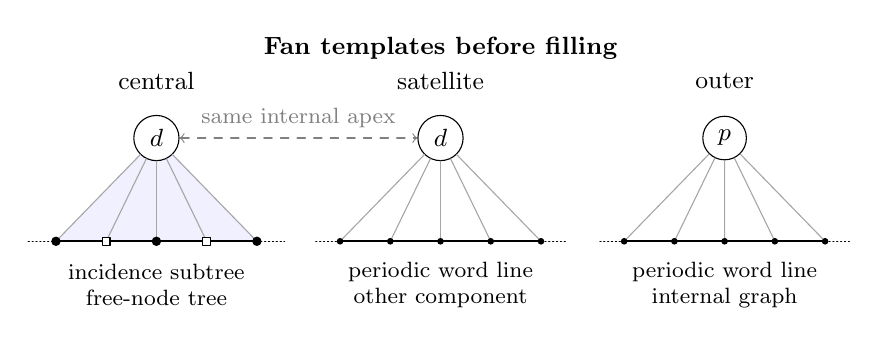
\begin{tikzpicture}[x=.88cm,y=.88cm,font=\small,
  every node/.style={align=center},line cap=round,line join=round,
  apex/.style={circle,draw,fill=white,inner sep=3pt},
  slot/.style={rectangle,draw,fill=white,inner sep=2pt}]
  \node[font=\small\bfseries] at (6,6.22)
    {Fan templates before filling};
  \node at (1.9,5.75) {central};
  \node at (6,5.75) {satellite};
  \node at (10.1,5.75) {outer};
  \fill[blue!6] (.45,3.43)--(1.9,4.92)--(3.35,3.43)--cycle;
  \node[apex] (dc) at (1.9,4.92) {$d$};
  \node[apex] (ds) at (6,4.92) {$d$};
  \node[apex] (po) at (10.1,4.92) {$p$};
  \draw[<->,dashed,gray] (dc)--node[above,font=\footnotesize]
    {same internal apex} (ds);
  \foreach \x in {.45,1.175,1.9,2.625,3.35} {
    \draw[gray!70] (dc)--(\x,3.43);
  }
  \draw[thick] (.45,3.43)--(3.35,3.43);
  \foreach \x in {.45,1.9,3.35} {\fill (\x,3.43) circle (1.7pt);}
  \foreach \x in {1.175,2.625} {
    \draw[fill=white] (\x-.055,3.375) rectangle (\x+.055,3.485);
  }
  \draw[densely dotted] (.05,3.43)--(.45,3.43);
  \draw[densely dotted] (3.35,3.43)--(3.75,3.43);
  \foreach \offset/\tip in {4.55/ds,8.65/po} {
    \draw[thick] (\offset,3.43)--(\offset+2.9,3.43);
    \draw[densely dotted] (\offset-.35,3.43)--(\offset,3.43);
    \draw[densely dotted] (\offset+2.9,3.43)--(\offset+3.25,3.43);
    \foreach \step in {0,.725,1.45,2.175,2.9} {
      \draw[gray!70] (\tip)--(\offset+\step,3.43);
      \fill (\offset+\step,3.43) circle (1.2pt);
    }
  }
  \node[font=\footnotesize,text width=3cm] at (1.9,2.8)
    {incidence subtree\\free-node tree};
  \node[font=\footnotesize,text width=3cm] at (6,2.8)
    {periodic word line\\other component};
  \node[font=\footnotesize,text width=3cm] at (10.1,2.8)
    {periodic word line\\internal graph};
\end{tikzpicture}
\caption{The three fan types before filling. The two $d$-symbols are
separate templates for one physical internal apex. Central fans cone
incidence subtrees in free-node Cayley trees; dots are ordinary sites and
small squares are horizontal midpoints. Satellite fans cone indexed word
lines mapping into other central components. Distinct satellite arms at
$d$ target distinct components in the developed model. An outer fan has
its own apex $p$ and an indexed word line mapping into the internal graph.
The word-line maps may repeat physical vertices and edges; their tags
retain the occurrences. The drawings are schematic and impose no planar
geometry.}
\label{fig:fan-templates}
\end{figure}


Let $K_J$ be the total kernel of the standalone induced filling of $J$,
and write
\[
 \overline{\mathcal X}=K_J\backslash\mathcal X,
 \qquad \mathcal A=\overline{\mathcal X}^{(1)}.
\]

\begin{lemma}[The filled model]\label{fan:filled-model}
For sufficiently deep choices, $\overline{\mathcal X}$ is simply
connected and $\mathcal A$ is uniformly hyperbolic.  The action of
$\bar J=J/K_J$ is cocompact, has free regular vertices and oriented
edges, and has exact finite apex stabilizers $\bar P=P/N_P$.
For each fixed filling, $\mathcal A$ is locally finite and proper, and
$\bar J$ is hyperbolic.

The central link $L_N(d)$ at an internal apex is the disjoint union of
its incidence subtrees modulo $N_P$.  Its components are exactly the
Stallings covers determined by $M\cap N_P$.  Satellite arms become
indexed path cycles of period $n=|\bar c|$; an outer apex has its one
indexed boundary cycle.  Period is measured in generator steps, with
bounded fractional offsets within the chosen word path.
\end{lemma}

\begin{proof}
The kernel $K_J$ is generated by conjugates of peripheral kernel
elements, each of which fixes an apex of $\mathcal X$.  A loop in the
quotient lifts edge by edge to a path upstairs with endpoint discrepancy
in $K_J$.  Express that discrepancy as a product of vertex-fixing
elements.  For each factor insert a path to its fixed apex followed by
the translated reverse path.  Its projection is a backtrack through
that apex.  The resulting closed path upstairs contracts because
$\mathcal X$ is simply connected.  This proves simple connectivity
of the quotient.

Exact peripheral reduction gives
$K_J\cap P=N_P$.  Two tags at a specified apex are consequently
identified precisely by $N_P$, proving the link assertion.  In
particular there is one apex for each marked coset, even when several
arms have that source.  Regular frame labels and oriented edge labels
become free $\bar J$-labels.  The arm stabilizer acts on its abstract
indexed line by its specified generator, so its quotient has exactly
$|\bar c|$ periods.

Formula~\eqref{fan:frame-formula} maps every edge to a bounded path in
the coned Cayley graph of the induced peripheral structure.  Conversely,
connectivity of $\mathcal X$ supplies fixed paths implementing its
finite relative generators, changing regular site types, and reaching
representatives of every apex orbit.  These paths descend, with bounds
independent of the filling.  Thus $\mathcal A$ and that coned Cayley
graph are uniformly quasi-isometric.  The relative filling bounds
from Section~\ref{sec:transfer-relative} give uniform hyperbolicity.  There
are finitely many edge orbits, free regular stabilizers, and finite
apex stabilizers, so a fixed quotient graph is locally finite and the
action is proper and cocompact.  It follows that $\bar J$ is hyperbolic;
its ordinary Cayley-metric comparison constants need not be uniform
as the filling varies.
\end{proof}

\subsection{Angles, tags, and exact covers}

For germs $e,e'$ at an apex $s$, define $\angle_s(e,e')$ to be the
shortest path length between their other endpoints in
$\mathcal A\setminus\{s\}$, with value $\infty$ if no such path exists.
Parallel tagged germs are distinguished even when this angle is zero.

\begin{lemma}[The finite angle dictionary]\label{fan:angle-dictionary}
All of the following conditions can be imposed for any finite list of
bounds before choosing the filling.
\begin{enumerate}[label=\textup{(\roman*)}]
\item There are no self-spokes.  Two distinct central spokes from a
fixed apex do not end at the same physical horizontal midpoint, and
likewise do not end at the same ordinary site.
\item For each $R$, after the first germ is normalized to a fixed
representative, every second germ at angle at most $R$ is obtained by a
translator from a fixed finite list in the original peripheral group.
The list includes the two germ types and does not depend on the filling.
Consequently angular balls have uniformly bounded cardinality.
\item On one indexed arm, source germs at bounded angle have sites
whose cyclic period coordinates differ by a uniformly bounded amount.
\item Every bounded closed walk in which each apex is visited at most
once cyclically has a closed labeled lift to the original fan graph,
with its given edge types and projected incidences.
\item All arm orders used here can be chosen even and arbitrarily
large.
\end{enumerate}
\end{lemma}

\begin{proof}
The first assertion holds upstairs.  Satellite targets belong to
components different from their source component.  Within the central
bipartite tree, at most one incidence joins a specified pair of nodes,
and its incidence subtree is embedded in the free tree.  A violation
after filling would give an equality of endpoint frames, or membership
of a fixed offset in a specified peripheral coset.  There are finitely
many edge types, so the finite-element and coset-avoidance tests from
Section~\ref{sec:transfer-relative} exclude these violations.

For the second assertion, expand an avoiding path in $\mathcal A$
using~\eqref{fan:frame-formula}.  Add its finitely many offsets to the
ordinary generating letters before setting the depth.  Each expanded
edge uses ordinary offsets and, when necessary, the cone legs at its
endpoints.  Neither endpoint is $s$.  Even when a germ's other endpoint
is a different apex, its connection to the designated ordinary germ
coordinate uses only fixed offsets and that other apex's cone leg.
Thus the expanded bypass still avoids the marked coset apex $s$.
Closing it across the two germs gives an isolated peripheral component.
The isolated-component bound for the uniformly linear relative
presentations, as used in Section~\ref{sec:transfer-relative}, places its
translator in a fixed finite set of actual peripheral elements
\cite{Osin2006,Osin2007}.  Tags and their free edge frames bound the
number of germs represented by that list.

For two sites on the same arm, normalize both word phases and write
the relative rotation as a power of its generator $c$.  The finite list
just obtained must lie in the image of $\langle c\rangle$.
Finite-list membership avoidance inside the ambient hyperbolic VCS
periodic peripheral ensures that such membership already holds before
filling.  Since $N_P$ lies inside the chosen base finite-index subgroup,
that test remains valid for the final kernel.  Each actual list element
then has a fixed exponent in $\langle c\rangle$, proving the period
bound.  For an outer cyclic peripheral this is immediate.  Word phases
only change the bound by a fixed amount.

For the fourth assertion, the rest of the closed walk is an avoiding
path at each of its apex visits.  Replace the successive normalized
peripheral transporters by elements of the finite lists in the second
assertion.  At regular vertices the transitions are fixed offsets.
After normalizing an initial oriented edge, the closing equation is
one of finitely many actual word equations.  Injection on that finite
set makes it hold upstairs.  This constructs one closed labeled lift;
it does not assert compatible lifts of arbitrarily many independent
translates.  That stronger assertion will not be needed.

Finally use the divisible order choices and exact order conclusions
of Proposition~\ref{kernel:orders}.  Only finitely many bounds and element
lists have been imposed, so all the choices are simultaneous.
\end{proof}

\begin{lemma}[Exact graph-cover data]\label{fan:cover-data}
Let $H_P$ be the intersection of a periodic peripheral's normal base
choice $H$ with $P_d$, and let $L_H(d)$ be its central link modulo
$H_P$.  Its finitely many components can be required to have
arbitrarily large girth.  Over each connected component $B$ there is a
nonempty finite collection of connected cyclic $\ell$-covers
$B_j\to B$, where $\ell>1$, and a finite field $\mathbb k$ with
$\operatorname{char}\mathbb k\nmid\ell$.  The corresponding component
of $L_N(d)$ is exactly the cover associated to the intersection of
\begin{enumerate}[label=\textup{(\roman*)}]
\item the kernels of all these cyclic covering maps; and
\item inside each covering kernel, the kernels of all additive first
cohomology classes in the nontrivial deck part of
$H^1(B_j;\mathbb k)$.
\end{enumerate}
The assertion holds also for the cyclic root incidences, whose
nontrivial deck cohomology part is zero.
\end{lemma}

\begin{proof}
Apply Corollary~\ref{kernel:graph-cover} to the actual free-row incidence
$M$.  In the unclaimed-root expansion, an elliptic $M_x^d$ is precisely
the corresponding free-edge-level incidence group, so the same
restriction theorem applies.  Its exact restriction statement is what
gives equality with the stated intersection, rather than merely a
cover factoring through it.  Conjugations and coset versions are
included in the kernel choices.  For root cyclic incidences use
Remark~\ref{kernel:cyclic-peripheral}: the character is surjective
modulo $\ell$ on the required intersection, and a cyclic group's first
cohomology has no nontrivial deck part.  Finally there are finitely many
original Stallings core types.  Residual finiteness of the ambient
periodic peripheral separates all their nonzero circuits of any fixed
length, giving the girth requirement before the character choices.
\end{proof}

\subsection{Large-angle comparisons}

We record the geometry used at each later wall gluing.  All constants
in this subsection depend on uniform hyperbolicity and the displayed
quasigeodesic constants, not on the final peripheral orders.

\begin{lemma}[Forced passage and marker comparison]
\label{fan:marker}\label{fan:marker-comparison}
In a uniformly hyperbolic graph the following hold.
\begin{enumerate}[label=\textup{(\roman*)}]
\item Geodesic legs from $s$ with sufficiently large angle concatenate
to a geodesic, and every geodesic between their other endpoints passes
through $s$.
\item Two uniform quasigeodesics from $s$ to the same finite or ideal
endpoint, neither revisiting $s$, have departure germs at bounded
angle.  If a geodesic has a sufficiently large interior angle at $s$,
a uniform comparison quasigeodesic cannot avoid $s$.  Nor can all its
germs at $s$ have a previously prescribed bounded angular diameter.
\item Suppose uniform quasi-isometrically embedded tree pieces are
joined by switches whose spokes have uniformly bounded lengths.
A switch maps to a marker in the graph.  For every reduced incidence
path, assume each connector through a piece has distinct endpoint
markers and avoids them except at its endpoints.  Impose the same
conditions on partial connectors at marked-node endpoints.  Assume
also that each piece attaches at most once at a given marker, and
that all distinct spoke germs at each switch have pairwise angle
larger than a sufficiently large fixed threshold.
Then the joined components are uniformly quasi-isometrically
embedded trees.  Their node projections are injective provided the
piece node projections are injective and the stated endpoint
conditions hold.  Every interior switch on a reduced path is a
large-angle turn on a geodesic between its projected endpoints.
The same conclusion holds towards an ideal endpoint of a ray when
the ambient graph is proper.
\end{enumerate}
The quasi-isometry constants in the third assertion can be fixed after
one minimum angle threshold is met.  Increasing the angle threshold
later increases the forced comparison angle without changing those
constants.
\end{lemma}

\begin{proof}
For the first two assertions use thin triangles and quasigeodesic
stability.  If a comparison path avoids $s$, choose points a sufficiently
large fixed distance out on the two relevant legs, using the endpoints
when a leg is shorter.  Thinness gives bounded bridges to the other
leg or to the comparison path.  Take the bridge points far enough
from $s$ that the bridges avoid it.  The portion of the comparison path
between the bridges has bounded length; for a quasigeodesic this follows
from its quasigeodesic inequality.  These paths give a bounded bypass
between the initial germs.  Thus a sufficiently large angle precludes
an avoiding geodesic and forces passage through $s$.  Its two subpaths
then have the lengths of the original legs, proving the concatenation
claim.  The same construction compares two departures to a common
endpoint.  For ideal endpoints first work on long finite initial
segments and use stability; properness supplies limiting geodesics
when required.  Finally, if the comparison path visits $s$, compare its
first and last visits towards the two endpoints.  A large geodesic
angle forces large angular diameter between these two comparison
germs.

For the gluing assertion, every piece connector is a uniform
quasigeodesic: adding bounded end spokes to a uniformly embedded
piece path changes only its additive constants.  The endpoint
avoidance hypotheses allow its departure and arrival germs to be
compared with those of a geodesic replacement.  The angle error is
bounded by the second assertion.  Hence consecutive replacement
geodesics still make an arbitrarily prescribed large angle at their
common switch if the spoke threshold is chosen sufficiently large.

Apply the first assertion inductively along a reduced incidence path.
The concatenation of its geodesic replacements is a geodesic, and
every interior switch remains a large-angle vertex on it.  A circuit
not contained in a piece would therefore give a positive-length
geodesic returning to its start; a circuit within a piece is impossible
because the piece is a tree.  Reusing one attachment does not create an
exception, since the incidence path was reduced and each piece has at
most one attachment at that marker.  The same argument rules out
repetition of node projections across switches; within pieces use the
assumed injectivity.

There are uniform constants $a,b$ such that the intrinsic length of
each connector is at most $a$ times the length of its geodesic
replacement plus $b$.  Distinct marker vertices have distance at least
one.  Summing over connectors therefore absorbs their additive errors
into a uniform multiplicative bound; the two end errors remain
uniformly bounded.  This proves quasi-isometric embedding.  Bounded
initial or terminal portions of spokes do not affect it.  Taking limits
proves the ray statement.  None of these estimates improves or worsens
when the angles are increased above the fixed minimum.
\end{proof}

\subsection{Sparse cuts from exact homological covers}

A \emph{central panel} $b$ at $d$ is a function
$\zeta_b:V(L_N(d))\to\{0,1\}$, defined on all ordinary link vertices.
Its \emph{cuts} are link edges with unequal endpoint labels.  The
corresponding cut germs are the central spokes to their midpoints.

\begin{proposition}[Central panel tests]
\label{fan:central-panels}\label{fan:sparse-panels}
Fix $K$, a bound $q$ on the number of target link vertices, and a bound
$r$ on the number of prescribed directions at an internal apex.
There is a bound $B$, depending only on these bounds and the fixed
original data, with the following property after suitable kernel
choices.  For every such target list and direction list there is a
partition of the targets into classes, each in one component of $L_N$
and of intrinsic diameter at most $B$, such that every binary
assignment to these classes extends to a central panel.  Its cut germs
are pairwise at angle greater than $K$, and all are at angle greater
than $K$ from the prescribed directions.  The same partition works
for all binary assignments.

There are also fillers: for every occurrence of a link edge there is
a panel cutting that occurrence whose cuts all lie over its one base
edge in $L_H$.  Its cut germs can be required pairwise farther than
$K$.
\end{proposition}

\begin{proof}
We first arrange that different lifts of any one edge of $L_H$ are
angularly farther than $K$.  Normalize their first tagged spoke by a
peripheral translator.  A short angle would, by
Lemma~\ref{fan:angle-dictionary}, give a translator from a fixed finite
actual list.  Since the lifts have the same image modulo $H_P$, its
image belongs to $H_P/N_P$.  Normality of $H$, and $N_P\le H_P$, put
the actual list element in $H_P$.  Choose $H$ to exclude all nonidentity
members of this list.  The remaining identity cannot identify two
different tagged spokes, whose stabilizers are trivial.

Select support base edges successively.  At each stage forbid all
base edges having a lift angularly near a prescribed direction or
near any lift of a support edge already chosen.  The number forbidden
by a direction is uniformly bounded.  The number forbidden by one
support edge is also uniformly bounded: the deck group $H_P/N_P$ is
transitive on all its tagged lifts, so normalize one lift and apply
the finite angle dictionary.  We will make at most $\binom q2$
selections.  There is consequently a uniform bound $B$ for the total
number of forbidden edges at every stage.  Enlarge $B$ if necessary
and require every $L_H$-component to have girth greater than $B$.
The forbidden-edge subgraph, including its isolated vertices, is then
a forest.

Here is the separation assertion underlying the construction.  Let
$u,v$ lie in one $L_N$-component, and let $F$ be its forbidden base
forest.  If $d_{L_N}(u,v)>B$, an allowed support edge supplies a
potential distinguishing them.  To prove this, choose a joining path
and project its chain to each cyclic cover $B_j$ from
Lemma~\ref{fan:cover-data}; call the chain $c_j$.  Put
\[
 A_j=\frac1\ell\sum_{g\in\operatorname{Deck}(B_j/B)}g
\]
for deck averaging on chains and cochains.  For each allowed base edge,
differences of the cochains on two of its individual oriented lifts
have coefficients $1,-1$ and lie in $\ker A_j$.  Their cohomology
classes belong to the nontrivial deck part.  Their pullbacks to $L_N$
are exact by the defining kernel property, hence are differentials
of $\mathbb k$-valued potentials.

Suppose none of these potentials distinguishes $u,v$.  Evaluation on
the projected path says that all coefficients of $c_j$ over any allowed
edge are equal.  Therefore
\begin{equation}\label{fan:forest-chain}
 (1-A_j)c_j\quad\hbox{is supported on the inverse image of }F,
 \qquad
 \partial(1-A_j)c_j=(1-A_j)([v_j]-[u_j]).
\end{equation}
Each lift of a base tree of $F$ is a tree, and there are $\ell$ such
lifts.  The augmentation of a boundary on each lifted tree is zero.
If the base projections of $u,v$ belonged to different base trees,
the right side of~\eqref{fan:forest-chain} would have nonzero
augmentation on at least one lift of either tree: its endpoint mass
is the difference between one point and its deck average, and
$\ell>1$ with $\ell$ invertible in $\mathbb k$.  The base endpoints
must therefore belong to one forest tree.  Their deck-average masses
on each lift cancel, so the same augmentation test forces $u_j,v_j$
to lie in the same lift of that tree.

Let $f$ be the unique base forest path between the two base endpoints.
It lifts to a path $f_j$ from $u_j$ to $v_j$ in every $B_j$.  The chains
$(1-A_j)c_j$ and $(1-A_j)f_j$ have the same boundary and are both
supported on a forest.  A forest has no nonzero one-cycles, so they
are equal.  Thus $c_j-f_j$ is invariant under deck averaging.  The
comparison loop belongs to every cyclic-cover kernel and evaluates
to zero on every nontrivial deck cohomology class.  Exactness in
Lemma~\ref{fan:cover-data} puts it in the final covering kernel.
Consequently $f$ lifts between the original $u,v$ in $L_N$, giving
$d_{L_N}(u,v)\le |F|\le B$, a contradiction.  This proves the
separation assertion.

Now process all same-component target pairs at distance greater than
$B$.  Select an allowed support edge and a distinguishing potential
for each pair still requiring distinction.  Extend each potential
constantly on the other components.  Two targets are put in the same
class precisely when they belong to the same component and have the
same tuple of potential values.  The separation assertion gives the
claimed diameter bound.  Any prescribed binary values on the target
classes extend to a binary function of this tuple and the component
identifier, assigning arbitrary values on the remaining tuples.
Its gradient is supported only over the selected support edges.
The forbidden-edge rule separates different support edges, while
the first paragraph separates different lifts of one support edge.
This proves both cut separation and avoidance of the direction list.

For a filler, choose a cyclic cover over the component in question
and take the difference cochain between the lift containing the
specified occurrence and a different lift of its base edge.  Its
pullback is exact and its value on the specified edge is nonzero.
A binary separation of the two endpoint potential values therefore
cuts that occurrence, with all cuts over that one base edge.  This
argument only requires the nontrivial covering degree.  In particular,
when the nontrivial cohomology itself is zero, the difference cochain
is already exact but still has a nonconstant potential.  The proof
works unchanged in characteristic two when $\ell$ is odd.
\end{proof}

\subsection{Central trees and their cochains}

For the actual finite links, take finite systems realizing all required
panel tests and then all peripheral translates.  Decorate panels by
free regular $\bar P_d$-multiplicities so that the data, rather than only
their isomorphism classes, translate equivariantly.  There are finitely
many requested orbits.  We next equalize their numbers of cuts.

For each central spoke orbit type, a peripheral orbit of fillers adds
a positive constant number of cuts at every spoke of that type and
none of the other types.  Multiply the requested systems by a common
multiple of these positive numbers.  Choose a common larger integer
$l$ divisible by all of them, and top up each type using its fillers.
Thus exactly $l$ cutting panels occur at every central spoke to a
midpoint.  The same $l$ can be used for all finitely many types.
Decorate every physical horizontal midpoint by $l$ slots, including
midpoints untouched by a particular panel system.  At each apex
incidence match the slots bijectively with its cutting panels.
Choose this matching equivariantly: the horizontal edge frames are
free, and Lemma~\ref{fan:angle-dictionary} gives only one central
occurrence from this apex at the specified midpoint.  Join a panel
to its assigned slots by edges projecting to its cut spokes.

\begin{lemma}[Central trees]\label{fan:central-trees}
Every component $W_0$ of the panel--slot graph is a uniformly
quasi-isometrically embedded tree in $\mathcal A$, injective on node
projections.  Its constants require only a minimum cut-angle threshold
and remain valid when subsequent panel systems use larger thresholds.
There are finitely many decorated node and edge orbits.  Distinct
systems may be retained separately as a finite labeled pool.
\end{lemma}

\begin{proof}
Apply Lemma~\ref{fan:marker} with slots as point pieces and panels as
switches.  Along a reduced path the two panel markers adjacent to one
slot are distinct: from a fixed apex, that slot is matched to only one
cutting panel.  The two-spoke connector through the slot avoids its
endpoint apices, and each point piece attaches at most once over any
apex.  At a panel all cut germs have the stipulated large angle.
The marker lemma proves both the tree assertion and injectivity on
nodes.  Finiteness of the orbit data follows from finite links, finite
peripheral reductions, and the finite multiplicities just chosen.
\end{proof}

A horizontal edge is \emph{marked by $W_0$} when its midpoint has a
slot in $W_0$, necessarily unique.  At an incident central link edge,
that slot belongs to $W_0$ precisely together with its matched cutting
panel.  There is at most one panel of $W_0$ above any given apex.

\begin{lemma}[The central cochain]\label{fan:central-cochain}
Each $W_0$ carries an equivariant mod-two cochain $\tau_0^{W_0}$ on the
central complex, closed on every central face.  It has value one on
the positive initial half of each marked horizontal edge, zero on all
other horizontal halves, and value $\zeta_b(t)$ on an ordinary radial
edge $d\!-\!t$ when its panel $b$ belongs to $W_0$, or zero when there
is no such panel.  Every edge with nonzero value has a panel or slot
anchor of $W_0$ at one of its endpoints.
\end{lemma}

\begin{proof}
The assertions specify the ordinary radial and horizontal values.
For an edge with positive orientation $u\!-\!m\!-\!v$, let
$\epsilon$ indicate whether it is marked.  Put the midpoint radial
value equal to $\zeta_b(u)+\epsilon=\zeta_b(v)$, taking the ordinary
radial labels to be zero if $b$ is absent.  The equality follows from
the matching rule: the link edge is a cut exactly when its slot and
cutting panel lie in this tree.  Both fan triangles therefore have
zero boundary sum.  These are all central faces.  The formulas also
give the anchor assertion and are preserved by the decorated group
action.
\end{proof}

\begin{lemma}[Satellite arm exclusivity and bounded support]
\label{fan:arm-exclusivity}
If $W_0$ has a node anchored on a satellite arm of $d$, then it has no
node over $d$ and no anchor on a different satellite arm of the same
$d$.  All its anchor occurrences on that arm, and all nonzero
occurrences of $\tau_0^{W_0}$ on its boundary cycle, lie in a period
interval of uniformly bounded diameter.  These bounds are independent
of the arm order and of later increases in cut separation.

If $\tau_0^{W_0}$ has odd total on the arm cycle, its stabilizer inside
$\bar P_d$ is trivial.
\end{lemma}

\begin{proof}
An anchor on the arm is joined to $d$ by its tagged source spoke.
If $W_0$ contained $d$, its intrinsic path to that anchor would have
uniformly bounded length by Lemma~\ref{fan:central-trees}.  Close it
by this spoke.  Likewise, anchors on two arms can be joined through
$d$ by two spokes, so their intrinsic $W_0$ path has uniformly bounded
length.  In the latter case $d$ has already been excluded.  These
closed walks are apex-simple: $W_0$ is injective on node projections
and its edges are central spokes, while the added source apex occurs
only at the cyclic joining point.  Lemma~\ref{fan:angle-dictionary}
therefore supplies a closed labeled lift upstairs.

The lift of the $W_0$ segment is a central path.  In the first case it
would join $d$ to a target component of its satellite arm, contrary to
Lemma~\ref{fan:components}.  In the second case it would join the
targets of two distinct arms in one central component.  The arms
remain distinct upstairs: at a fixed source, their incidence tags
are cosets $P_d/\langle c\rangle$, and the quotient construction gives
the corresponding cosets in $\bar P_d$.  If two lifted incidences
were the same, their projected incidences would be the same.  Thus one
closed polygon lift suffices for this contradiction; no simultaneous
lifting of independently chosen translates is being assumed.

The path in $W_0$ between two anchors on the one remaining arm has
bounded length, using the two-spoke shortcut through $d$, and avoids
$d$.  Apply the period part of Lemma~\ref{fan:angle-dictionary} to
obtain the bounded interval.  A nonzero central cochain occurrence
has an anchor at an endpoint, and the word paths have fixed lengths,
so a fixed enlargement of this interval contains its support.

An odd total makes the support nonempty.  Any element of $\bar P_d$
stabilizing $W_0$ must preserve its unique encountered arm.  That arm's
stabilizer acts faithfully by rotations of its tagged period cycle.
For order sufficiently large compared with the support diameter, no
nonidentity subgroup of this rotation group preserves a nonempty
subset contained in such a short interval.  This proves the last
assertion.  All bounds used the minimum quasi-isometry constants and
fixed word lengths, so increasing the cut threshold does not change
them.
\end{proof}

\subsection{Odd seeds on satellite arms}

\begin{proposition}[Odd inner seeds]\label{fan:odd-seeds}
A finite pool of central panel systems, chosen at successive fixed
angle scales, can be required to contain, on every satellite arm, a
central tree $W_0$ for which $\tau_0^{W_0}$ has odd total on the arm's
boundary cycle.  The choices and all support bounds are independent
of the sufficiently large individual cycle orders.
\end{proposition}

\begin{proof}
Fix an arm cycle $\beta$ with source $d$ and period $n$.
At each internal apex $s$ visited by its central boundary path, list
all radial half-incidences, with multiplicity.  Their other endpoints
are ordinary by construction.  The list size is uniformly bounded:
all source spokes from $d$ to the repeated occurrence of $s$ have the
same other endpoint, hence angle zero at $d$; the finite angle
and period dictionaries bound both their number and their period
spread.  At $s$ the listed directions are mutually close in angle by
paths through $d$.

Use Proposition~\ref{fan:central-panels} with cuts sufficiently far
from these directions and with every binary assignment on its bounded
diameter target classes.  For the tree through such a testing panel
at $s$, no other anchor $w\ne s$ lies on $\beta$.  Indeed the arm
exclusivity lemma excludes $d$ from this tree.  Its path from $s$ to
$w$ can be compared with the path $s\!-\!d\!-\!w$ of length at most
two.  The first germ of the latter is close to every listed direction
at $s$, by the adjacent ordinary site on $\beta$.  Departure comparison
in Lemma~\ref{fan:marker} contradicts the first cut's chosen distance
from those directions.  The cochain's total on $\beta$ is therefore
exactly the sum of the tested labels at $s$.

If any test has odd total, it supplies the seed.  Otherwise every
target class occurs an even number of times.  Pair the radial
half-incidences within each class and replace each pair, as a mod-two
chain, by a horizontal link path between its two ordinary sites.
The paths have a uniform length bound $B_1$.  Fan triangles show that
each replacement preserves evaluation by every central cochain.
Perform this at all visited apices.  The result is a finite purely
horizontal cycle chain $z$; connectivity is not required.

We justify that $z$ is nonzero by retaining its winding around the
period circle $C_n=\mathbb R/n\mathbb Z$.  Initially each occurrence
on $\beta$ has its indexed period coordinate, with the fixed
fractional coordinates inside a word.  Every vertex occurrence added
by a replacement has a horizontal tail of length at most $B_1$ to
one of the original ordinary sites.  Two occurrences representing the
same physical vertex thus have original sites joined by a bounded
path avoiding $d$.  Their source spokes have bounded angle at $d$,
so their period coordinates differ by a fixed bounded amount.
The same applies to the two occurrences of $s$ involved in each
paired replacement.  Consequently each replacement polygon, and
all ambiguity in assigning coordinates to one physical vertex,
occupies a period interval of bounded diameter.

For completeness, let $T$ bound horizontal replacement lengths in
our subdivided metric, and let $D(R)$ be the period-coordinate bound
for original occurrences joined by a path of length at most $R$
avoiding $d$.  Enlarge it monotonically and put
\[
 M=\max\{1,D(T),D(2T+1)\},\qquad n>8M.
\]
For every physical vertex in the finite graph used by $\beta$ and
the replacements, choose one original occurrence reachable by a
horizontal tail of length at most $T$, and assign its period
coordinate to the vertex.  Original vertices, including apices,
allow the zero-length tail.  Map each physical edge by the unique
short arc between its assigned endpoint coordinates.  The assigned
coordinate at an original occurrence differs from its parameter
coordinate by at most $M$.  Along the indexed original cycle choose
these errors in $[-M,M]$.  Each elementary parameter increment is
at most one, so its adjusted increment has absolute value at most
$1+2M<n/2$ and is exactly the chosen short-arc increment.  The errors
telescope around the cycle, leaving total increment $n$ and degree
one.  For a replacement polygon centered at an occurrence of $s$,
the witness original occurrence of any of its vertices is joined
to that $s$ by an avoiding path of length at most $2T+1$.
All assigned coordinates therefore lie in one interval of length
at most $2M<n/2$.  Its edge images stay in that interval, so the
polygon has degree zero.  The image of
$z$ thus has degree one modulo two.  In particular some physical
horizontal edge occurs in $z$ with coefficient one.  At its midpoint
the cycle equation makes the two half-edge coefficients equal.

Choose a second central panel system with cut angles larger than a
threshold fixed after $B_1$, and take the central tree through a slot
of that edge.  It has no node above $d$.  Otherwise close its bounded
path to the slot by the slot's bounded horizontal tail to an original
arm site and the source spoke to $d$.  The added tail has no apices,
so the resulting bounded walk is apex-simple and lifts by
Lemma~\ref{fan:angle-dictionary}.  Its lifted central path would join
$d$ to the target component, the contradiction used in
Lemma~\ref{fan:arm-exclusivity}.

Nor can this tree contain two distinct horizontal anchors of $z$.
Each anchor has a bounded horizontal tail to $\beta$, and hence a
bounded path to $d$.  Between two distinct slot nodes the tree path
has an interior panel marker, different from $d$.  Its angle is larger
than the fixed comparison threshold.  The path between the two
anchors formed from their horizontal tails and the two source spokes
through $d$ has uniformly bounded length and avoids every such marker.
It is a uniform comparison quasigeodesic, with constants depending
only on that length bound.  Lemma~\ref{fan:marker} gives a
contradiction.  Thus the chosen tree has exactly one horizontal anchor
on the support of $z$.  Its cochain evaluates to one there, and hence
to one on $z$ and on the original $\beta$.

There are only finitely many actual links and bounded-size requests
for a fixed filling.  Include all first-stage tests, their translates,
and the second-stage filler systems.  The constants determining these
requests were fixed independently of $n$, so this is a finite pool
working for every sufficiently deep filling and every arm type.
\end{proof}

\subsection{Order and uniformity of the choices}\label{fan:scale-order}

We make explicit the quantifier order used here and in the next
section.  First fix the original row types, their word paths, the
uniform relative hyperbolicity bounds, and a minimum bend threshold
in Lemma~\ref{fan:marker}.  This fixes the quasi-isometry constants of
the central trees and the arm-support bounds in
Lemma~\ref{fan:arm-exclusivity}.  Any larger cut separations preserve
these constants.

Next prescribe the finitely many target-list sizes and direction
avoidance thresholds that will be tested.  Proposition~\ref{fan:central-panels}
provides a bound for the number of forbidden base edges and for the
resulting class diameters, independently of $H$ and $N_P$.  For odd
seeds, choose the first testing threshold, compute its replacement
bound $B_1$, and only then choose the second cut threshold needed to
exclude the bounded comparison paths.  The two systems remain
separately tagged: the first-stage class bound is not recomputed
using the second threshold.  All angle dictionaries and
short-polygon lifting tests at these finitely many scales are now
fixed.  Subsequent applications may repeat this finite procedure,
provided each new threshold depends only on already fixed bounds.

Finally choose the normal base subgroups $H$ to meet all resulting
finite-list exclusions and girth bounds.  Apply the character and
cohomology kernel construction, preserving those tests because
$N_P\le H_P$.  Choose the cyclic orders even and larger than the
finitely many period and support bounds.  The graph-cover argument
uses the number of target pairs, not the number of characters or the
size of a final link, so enlarging a cover at this last stage does not
alter any previously fixed bound.  All these choices are compatible
with any initial finite-path filling requirements by
Proposition~\ref{kernel:construction}.

The outgoing data are therefore a finite pool of equivariant central
trees $W_0$, their central cocycles $\tau_0$, arbitrary prescribed panel
tests of the stated bounded type, and odd inner seeds with uniformly
bounded support and free arm stabilizers.  These are the data used to
attach the satellite and outer switches.
